\subsection{Seq2Seq3BiLSTM}
La classe \texttt{Seq2Seq3BiLSTM} implementa un'architettura simile al modello Seq2SeqBiLSTM, ma con tre layer LSTM bidirezionali nell'encoder.\\
Di seguito, possiamo vedere un diagramma dell'architettura del modello Seq2Seq3BiLSTM nella figura \ref{fig:seq2seq3bilstm_model_architecture}.
\begin{figure}[H]
    \centering
    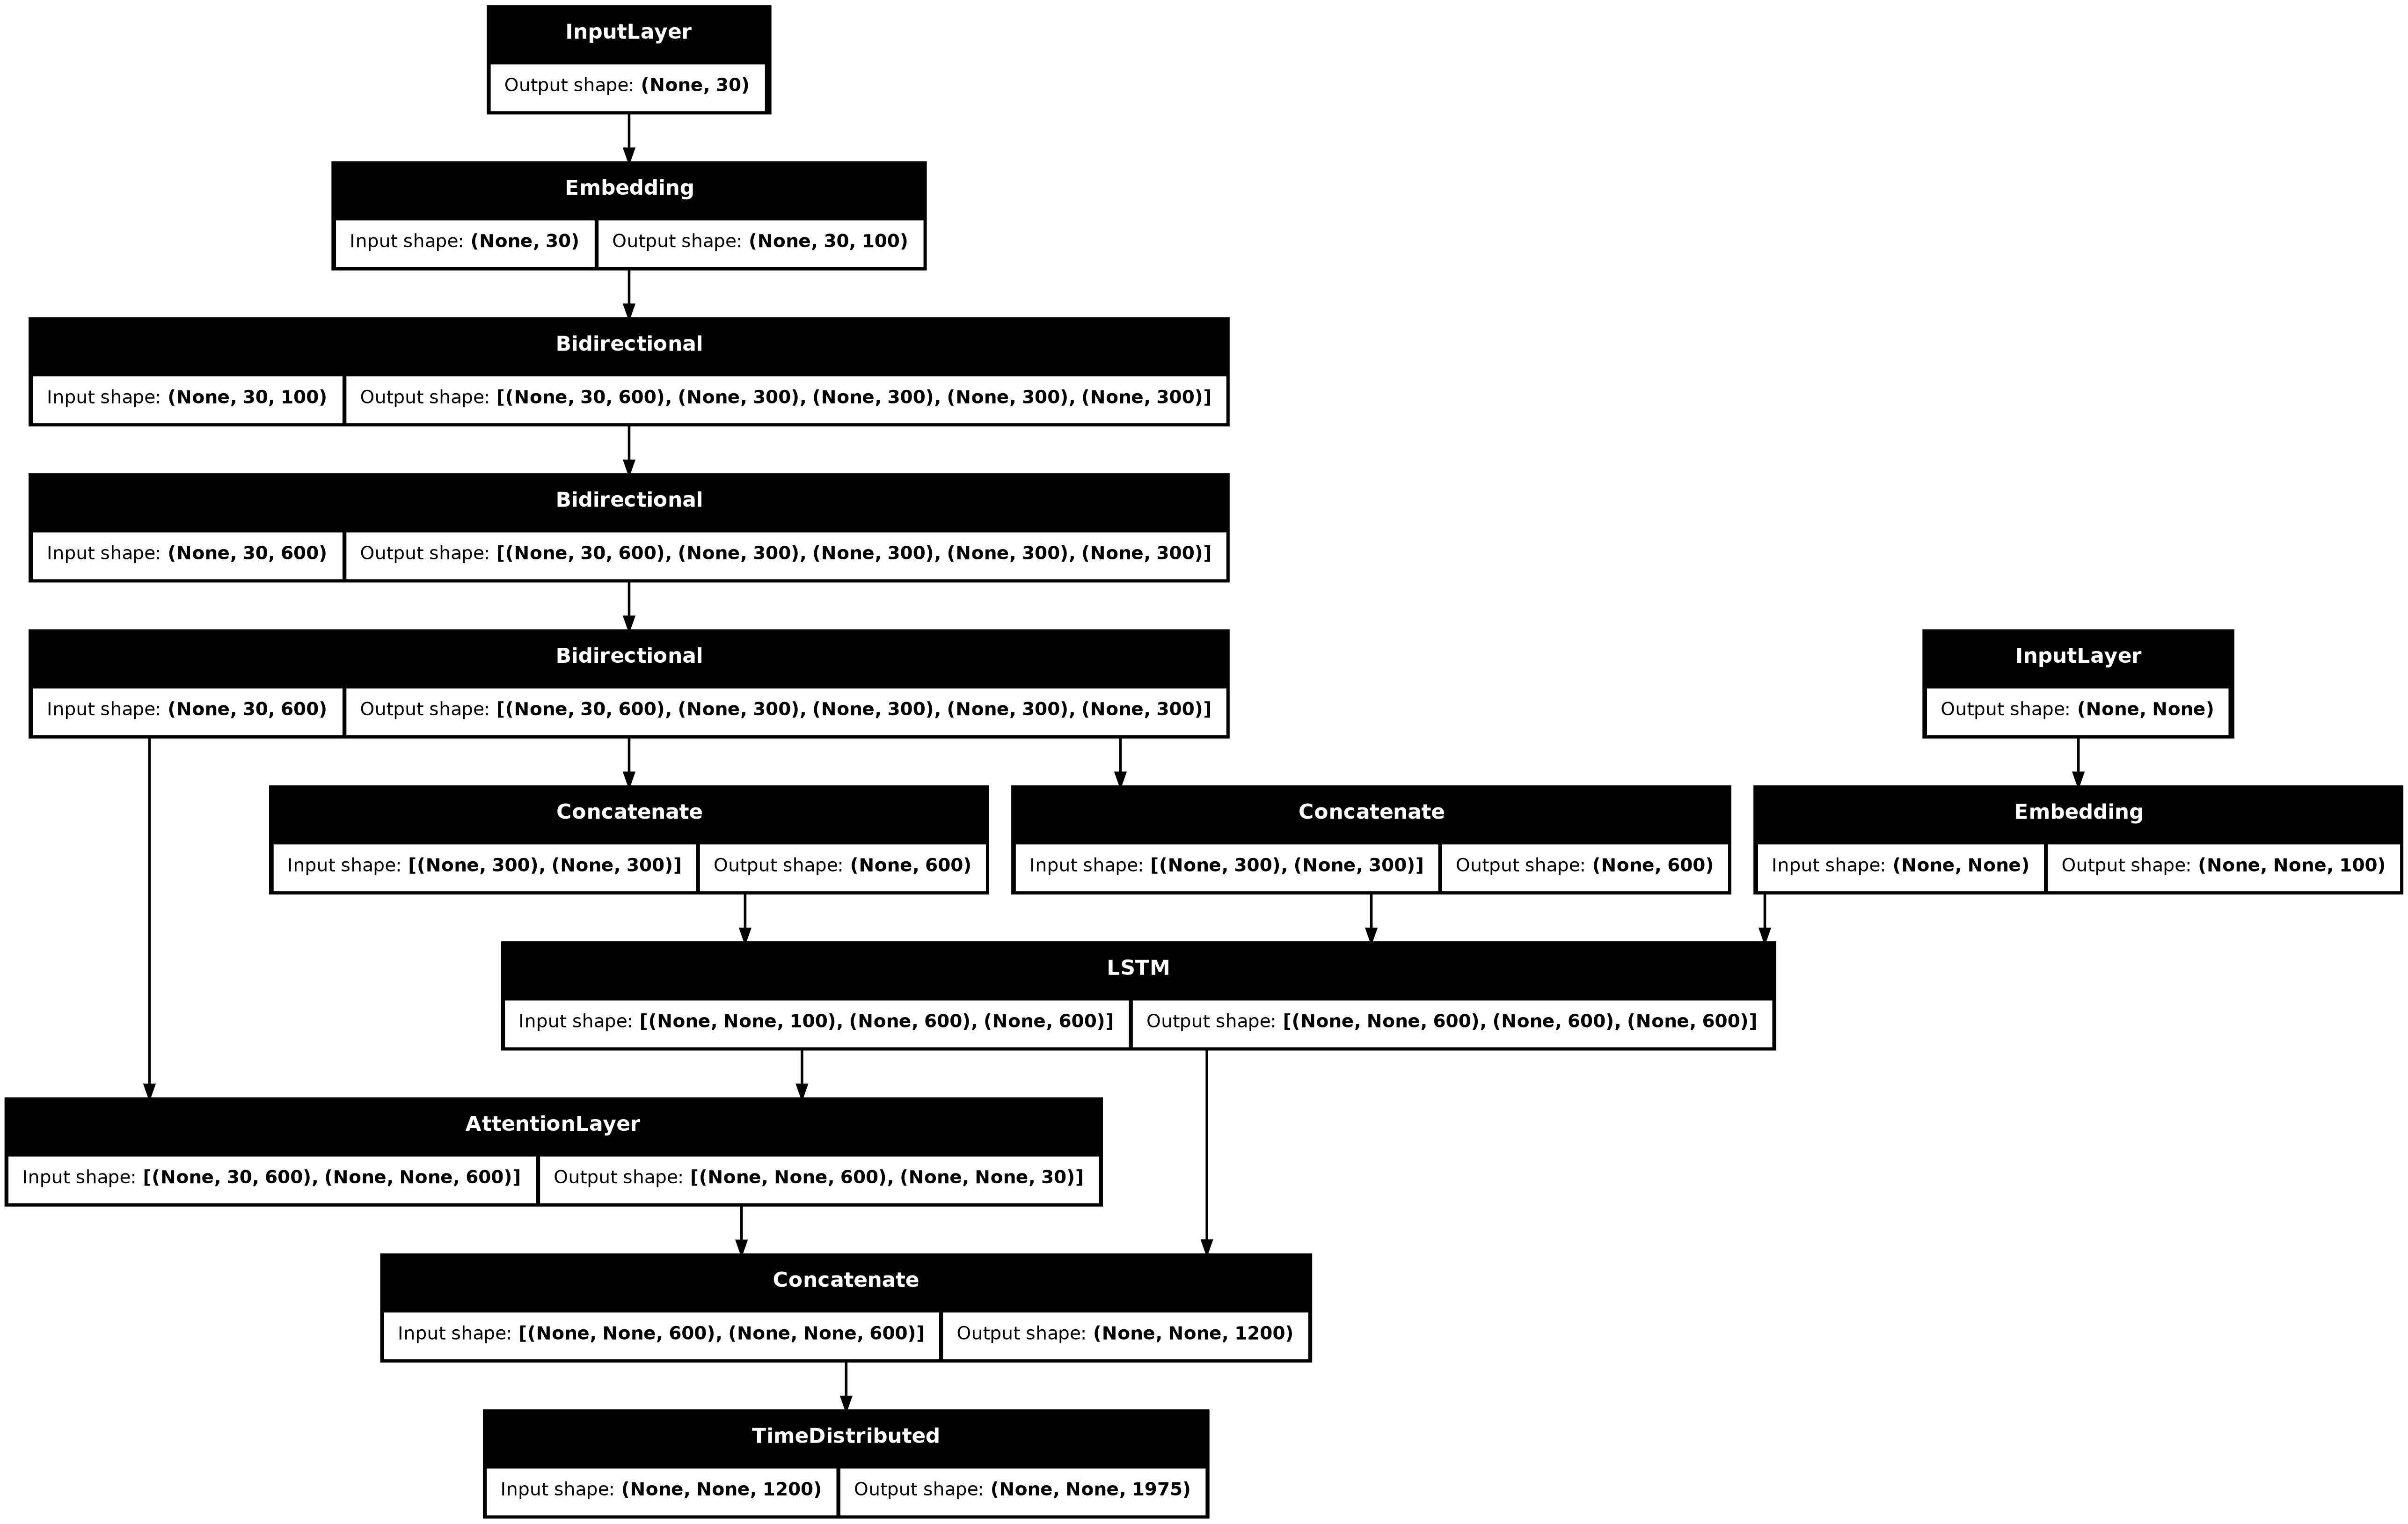
\includegraphics[width=1\textwidth]{media/Seq2Seq3BiLSTM_image.png}
    \caption{Diagramma dell'architettura del modello Seq2Seq3BiLSTM}
    \label{fig:seq2seq3bilstm_model_architecture}
\end{figure}

\training{Adam}{50}
\risultati{DA INSERIRE}{DA INSERIRE}{DA INSERIRE}{DA INSERIRE}

\begin{figure}[H]
    \centering
    %TODO: Aggiungere immagine traingin loss È DA AGGIORNARE
    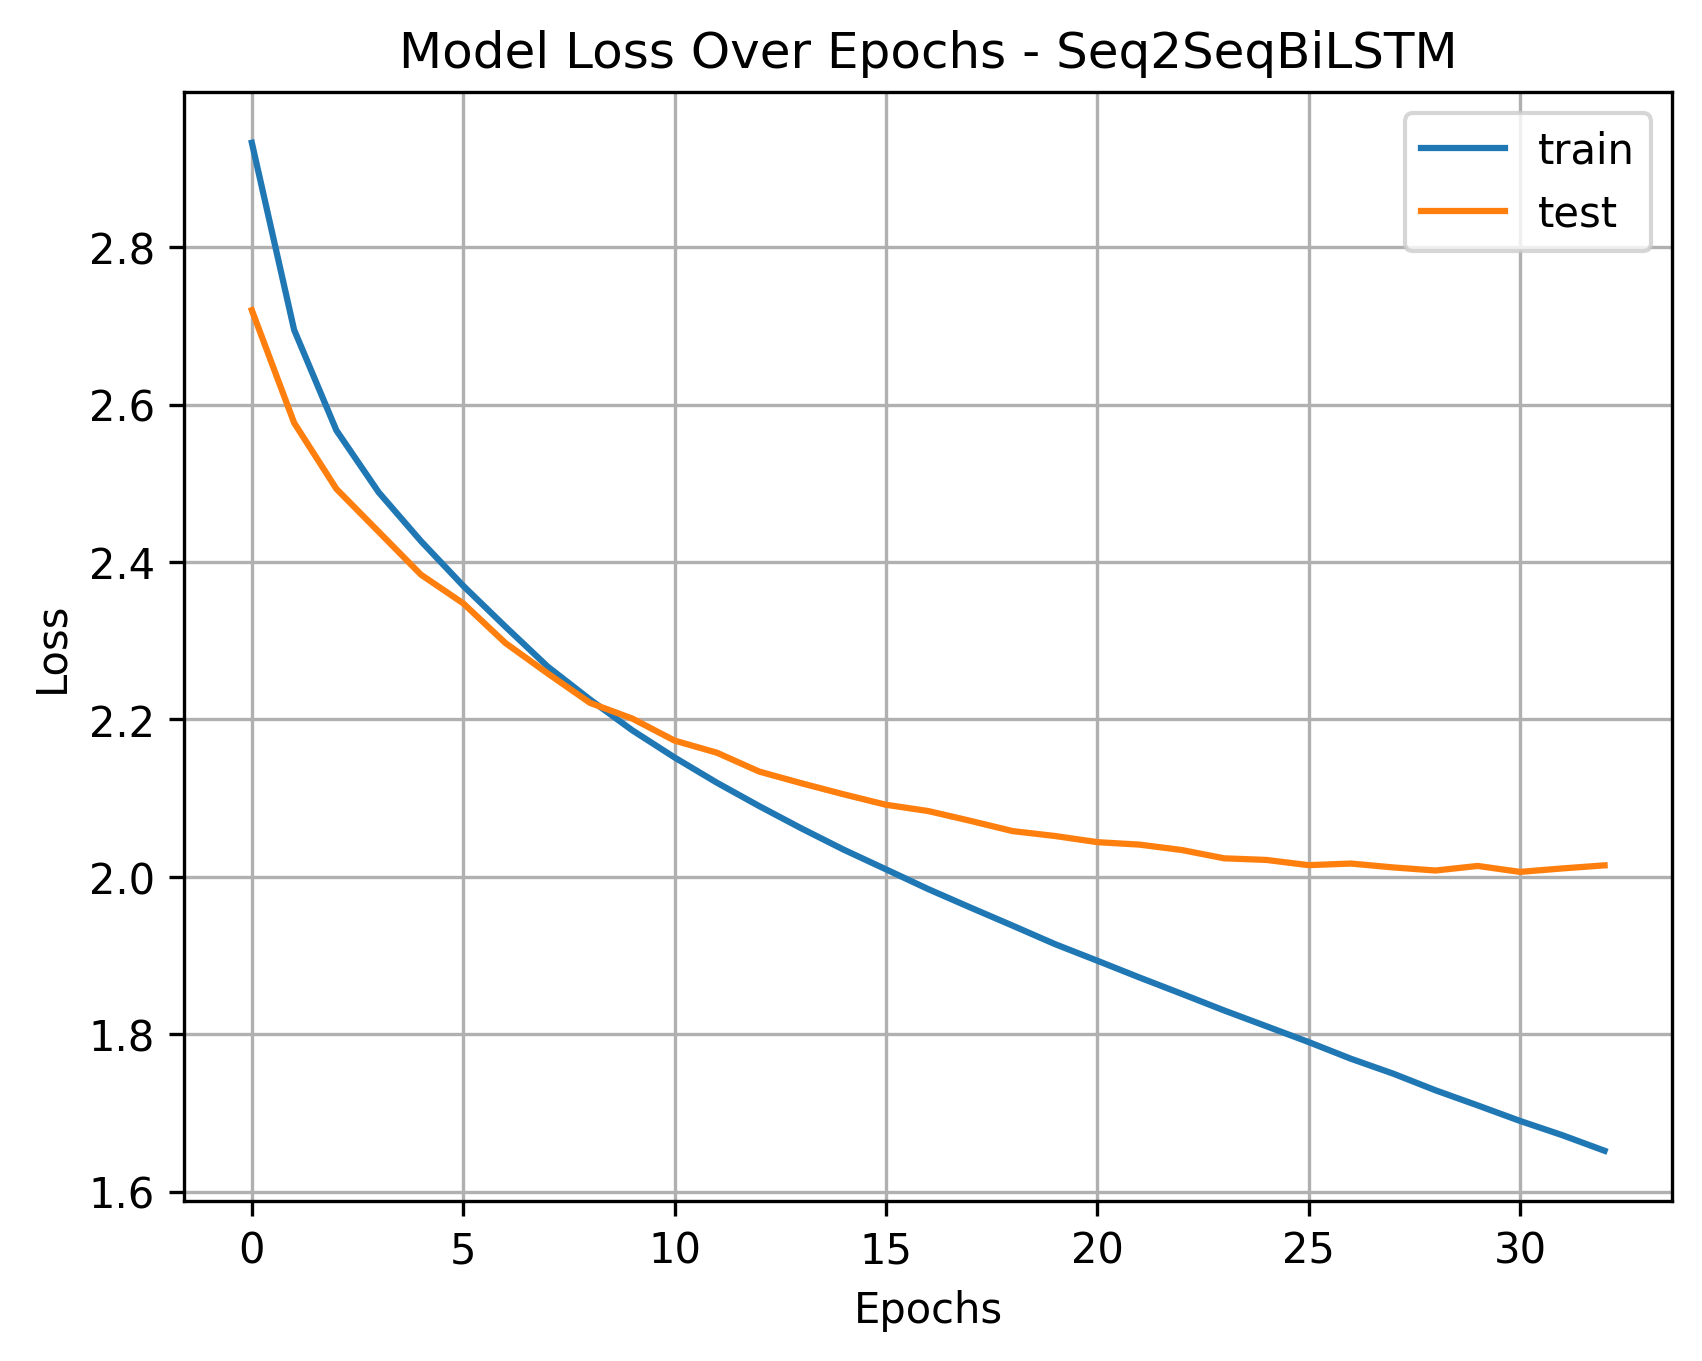
\includegraphics[width=0.75\textwidth]{media/Seq2Seq3BiLSTM_originale_lossplot.png}
    \caption{Andamento delle loss durante l'addestramento}
    \label{fig:seq2seq3bilstm_loss_plot}
\end{figure}

